\section{Basic}
	\subsection{vimrc}
		=== .vimrc 	===
\lstinputlisting{Basic/vimrc/.vimrc}

	\subsection{default code}
		\lstinputlisting{Basic/T.cpp}
	\subsection{state machine}
		\begin{center}
		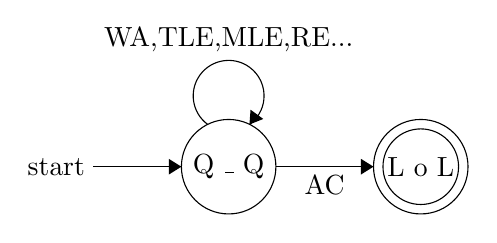
\begin{tikzpicture}[scale=0.2]
		\tikzstyle{every node}+=[inner sep=0pt]
		\draw [black] (29.5,-22.7) circle (3);
		\draw (29.5,-22.7) node { L o L };
		\draw [black] (29.5,-22.7) circle (2.4);
		\draw [black] (17.3,-22.7) circle (3);
		\draw (17.3,-22.7) node {Q \_ Q};
		\draw [black] (15.977,-20.02) arc (234:-54:2.25);
		\draw (17.3,-15.45) node [above] {WA,TLE,MLE,RE...};
		\fill [black] (18.62,-20.02) -- (19.5,-19.67) -- (18.69,-19.08);
		\draw [black] (8.7,-22.7) -- (14.3,-22.7);
		\draw (8.2,-22.7) node [left] {start};
		\fill [black] (14.3,-22.7) -- (13.5,-22.2) -- (13.5,-23.2);
		\draw [black] (20.3,-22.7) -- (26.5,-22.7);
		\fill [black] (26.5,-22.7) -- (25.7,-22.2) -- (25.7,-23.2);
		\draw (23.4,-23.2) node [below] {AC};
		\end{tikzpicture}
		\end{center}
		\begin{center}
		    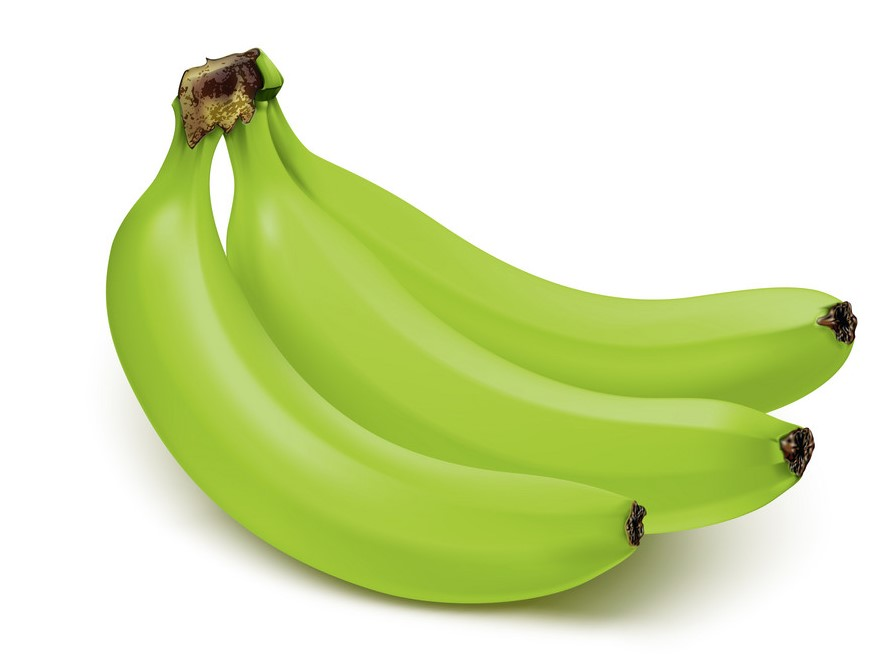
\includegraphics[scale=0.3]{logo.jpg}
		\end{center}
		\newpage

\section{Flow}
	\subsection{Dinic}
		\lstinputlisting{Graph/Flow/dinic.cpp}
	\subsection{GomoryHu tree 全點對最小割DC法}
		\lstinputlisting{Graph/Flow/Gomory_Hu.cpp}
%	\subsection{Karzanov}
%		\lstinputlisting{Graph/Flow/Karzanov.cpp}
	\subsection{min cost flow}
		\lstinputlisting{Graph/Flow/Min_Cost_Max_Flow.cpp}
	\subsection{SW mincut 全點對最小割}
		\lstinputlisting{Graph/Flow/SW-mincut.cpp}


\section{Matching}
	\subsection{Hungarian}
		\lstinputlisting{Graph/Matching/Hungarian.cpp}
	\subsection{KM}
		\lstinputlisting{Graph/Matching/Kuhn_Munkres.cpp}
	\subsection{Matching.txt}
		\lstinputlisting{Graph/Matching/Matching.txt}
	\subsection{Maximum General Matching}
		\lstinputlisting{Graph/Matching/Maximum_General_Matching.cpp}
	\subsection{Minimum General Weighted Matching}
		\lstinputlisting{Graph/Matching/Minimum_General_Weighted_Matching.cpp}


\section{Graph}
		\begin{itemize}
\item Maximum Independent Set 
	\begin{itemize}
	\item General: [NPC] maximum clique of complement of G
	\item Bipartite Graph: [P] Maximum Cardinality Bipartite Matching
	\item Tree: [P] dp
	\end{itemize}
\item Minimum Dominating Set
	\begin{itemize}
	\item General: [NPC]
	\item Bipartite Graph: [NPC]
	\item Tree: [P] DP
	\end{itemize}
\item Minimum Vertex Cover
	\begin{itemize}
	\item General: [NPC] (?)maximum clique of complement of G 
	\item Bipartite Graph: [P] Maximum Cardinality Bipartite Matching
	\item Tree: [P] Greedy, from leaf to root
	\end{itemize}
\item Minimum Edge Cover
	\begin{itemize}
	\item General: [P] V - Maximum Matching
	\item Bipartite Graph: [P] Greedy, strategy: cover small degree node first.
	\item (Min/Max)Weighted: [P]: Minimum/Minimum Weight Matching
	\end{itemize}
\end{itemize}
	\subsection{BCC edge}
		\lstinputlisting{Graph/BCC_edge.cpp}
	\subsection{Dijkstra}
		\lstinputlisting{Graph/Dijkstra.cpp}
%e	\subsection{Dijkstra (python)}
%		\lstinputlisting{Graph/Dijkstra.py}
	\subsection{Domination.txt}
		\lstinputlisting{Graph/Domination.txt}
%?	\subsection{Dominator tree}
%		\lstinputlisting{Graph/DominatorTree.cpp}
%?	\subsection{Kosaraju SCC}
%		\lstinputlisting{Graph/Kosaraju_SCC.cpp}
	\subsection{LCA}
		\lstinputlisting{Graph/LCA.cpp}
	\subsection{max clique}
		\lstinputlisting{Graph/MaximumClique.cpp}
	\subsection{min mean cycle}
		\lstinputlisting{Graph/Min_mean_cycle.cpp}
%?	\subsection{min Steiner tree}
%		\lstinputlisting{Graph/MinimumSteinerTree.cpp}
%?	\subsection{SchreierSims}
%		\lstinputlisting{Graph/SchreierSims.cpp}
	\subsection{SSSP related concepts}
		\lstinputlisting{Graph/SSSP-related-concepts.txt}
	\subsection{Tarjan.cpp}
		\lstinputlisting{Graph/Tarjan.cpp}
	\subsection{2-SAT}
		\lstinputlisting{Graph/TwoSAT.cpp}
	\subsection{平面圖判定}
		\lstinputlisting{Graph/planar.cpp}


\section{Math}
		\begin{itemize}
\item Stirling number of second kind \\
	\( S(n,m)\) :  n 個相異球, 放到 m 個相同的相子, 每個箱子至少 1 \\
	\( = m \times S(n-1,m) + S(n-1,m-1) \) \\
	\( = \frac{1}{m!} \sum_{j=0}^{m} \binom{m}{j} (m-j)^n (-1)^j \)
\item Stirling number of first kind \\
	\( s(n,m)\) :  n 個相異球, 分配到 m 個有向環, 每個環至少 1 \\
	\( s(n+1,m) = n \times s(n,m) + s(n,m-1) \) \\
	\( s(n,m) \equiv \binom{ \left \lfloor n/2 \right \rfloor }{ m-\left \lfloor n/2 \right \rfloor }\) mod 2
\item Pick's Theorem (Bangkok regional 2016 pD) \\
	多邊形頂點都在整數點上 \\
    多邊形面積 = 內部整數點個數 + 邊上格子點個數/2 - 1\\
	\( A = i + b/2 -1 \)
\end{itemize}
	\subsection{ax+by=gcd(a,b)}
		\lstinputlisting{Math/ax+by=gcd.cpp}
%e	\subsection{Bigint}
%		\lstinputlisting{Math/Bigint.cpp}
	\subsection{FFT}
		\lstinputlisting{Math/FFT.cpp}
	\subsection{NTT}
		\lstinputlisting{Math/NTT.cpp}
%e	\subsection{FWHT}
%		\lstinputlisting{Math/FWHT.cpp}
	\subsection{GaussElimination}
		\lstinputlisting{Math/GaussElimination.cpp}
	\subsection{inverse}
		\lstinputlisting{Math/inverse.cpp}
%e	\subsection{Karatsuba}
%		\lstinputlisting{Math/Karatsuba.cpp}
%e	\subsection{LinearPrime}
%		\lstinputlisting{Math/LinearPrime.cpp}
	\subsection{Miller-Rabin}
		\lstinputlisting{Math/Miller-Rabin.cpp}
	\subsection{Mobius}
		\lstinputlisting{Math/Mobius.cpp}
	\subsection{pollardRho}
		\lstinputlisting{Math/pollardRho.cpp}
%e	\subsection{Random}
%		\lstinputlisting{Math/Random.cpp}
	\subsection{SG}
		\lstinputlisting{Math/Sprague-Grundy.cpp}
	\subsection{theorem}
		\lstinputlisting{Math/theorem.cpp}

\section{Geometry}
	\subsection{2D point template}
		\lstinputlisting{Geometry/2Dpoint.cpp}
	\subsection{circumcentre}
		\lstinputlisting{Geometry/circumcentre.cpp}
	\subsection{ConvexHull}
		\lstinputlisting{Geometry/ConvexHull.cpp}
	\subsection{3D ConvexHull}
		\lstinputlisting{Geometry/3D_ConvexHull.cpp}
	\subsection{half plane intersection}
		\lstinputlisting{Geometry/half_plane_intersection.cpp}
	\subsection{Intersection of two circle}
		\lstinputlisting{Geometry/Intersection_of_two_circle.cpp}
	\subsection{Intersection of two lines}
		\lstinputlisting{Geometry/Intersection_of_two_lines.cpp}
	\subsection{Smallest Circle}
		\lstinputlisting{Geometry/Smallest_Circle.cpp}

\section{String}
	\subsection{AC automaton}
		\lstinputlisting{String/AC.cpp}
	\subsection{KMP}
		\lstinputlisting{String/KMP.h}
	\subsection{palindromic tree}
		\lstinputlisting{String/PalindromicTree.cpp}
	\subsection{SAM}
		\lstinputlisting{String/SAM.cpp}
	\subsection{smallest rotation }
		\lstinputlisting{String/smallest_rotation.cpp}
	\subsection{suffix array}
		\lstinputlisting{String/suffix_array.cpp}
	\subsection{Z value}
		\lstinputlisting{String/Z-value.cpp}
	\subsection{BWT (Burrows-Wheeler Transform)}
		\lstinputlisting{String/BWT.cpp}

\section{Data structure}
	\subsection{2D range tree}
		\lstinputlisting{DataStructure/2D_RangeTree.cpp}
	\subsection{ext heap}
		\lstinputlisting{DataStructure/ext_heap.cpp}
	\subsection{KD tree}
		\lstinputlisting{DataStructure/KDTree.cpp}
	\subsection{Link-Cut tree}
		\lstinputlisting{DataStructure/link_cut_tree.cpp}
%e	\subsection{sparse table}
%		\lstinputlisting{DataStructure/SparseTable.h}
	\subsection{Treap}
		\lstinputlisting{DataStructure/Treap.cpp}
%	\subsection{Treap Lin}
%		\lstinputlisting{DataStructure/Treap_Lin.cpp}

\section{Other}
	\subsection{count spanning tree}
		\lstinputlisting{Other/count_spanning_tree.cpp}
	\subsection{C++11 random}
		\lstinputlisting{Other/CppRandom.cpp}
%e	\subsection{CYK}
%		\lstinputlisting{Other/CYK.cpp}
	\subsection{Digit Counting}
		\lstinputlisting{Other/DigitCounting.cpp}
	\subsection{DP optimization}
		\lstinputlisting{Other/DP-optimization.txt}
	\subsection{DP 1D/1D}
		\lstinputlisting{Other/Dp1D1D.cpp}
%n	\subsection{IO optimization}
%		\lstinputlisting{Other/IO_optimization.cpp}
	\subsection{Manhattan MST.cpp}
		\lstinputlisting{Other/ManhattanMST.cpp}
	\subsection{stable marriage}
		\lstinputlisting{Other/Marriage.cpp}
	\subsection{Mo's algorithm}
		\lstinputlisting{Other/Mo_algorithm.cpp}
	\subsection{Parser}
		\lstinputlisting{Other/Parser.cpp}
	\subsection{python cheat sheet}
		\lstinputlisting{Other/python.py}
\onecolumn
\centering
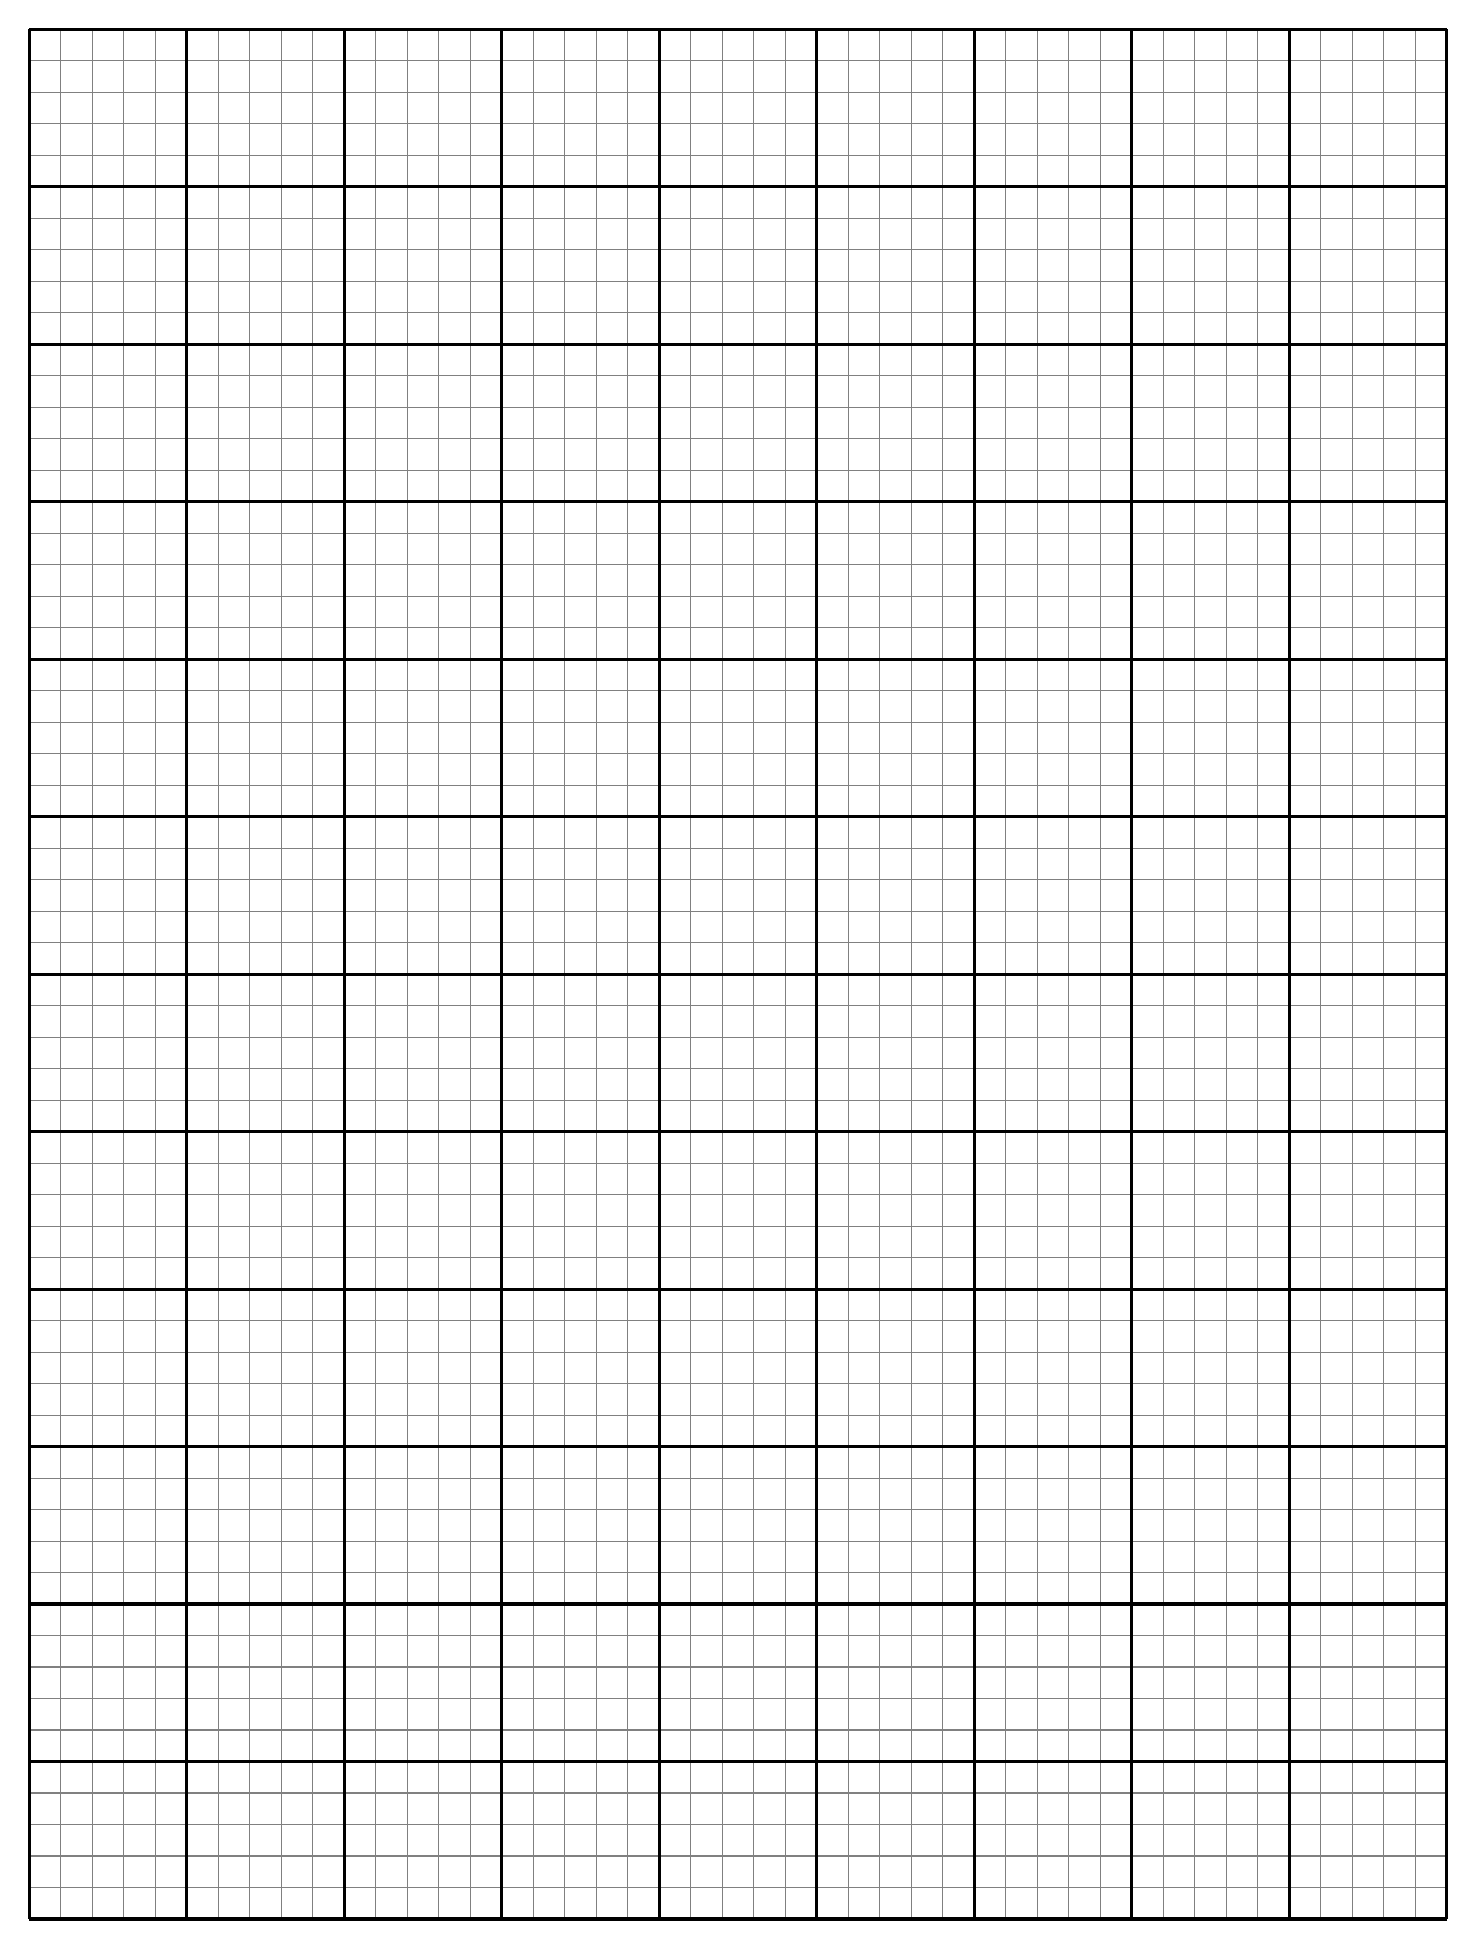
\begin{tikzpicture}[every node/.style={minimum size=1cm-\pgflinewidth, outer sep=10pt}, scale=2]
    \draw[step=0.2cm,color=gray] (0,0) grid (9,12);
    \draw[step=1cm,color=black,line width=0.4mm] (0,0) grid (9,12);
\end{tikzpicture}

\centering
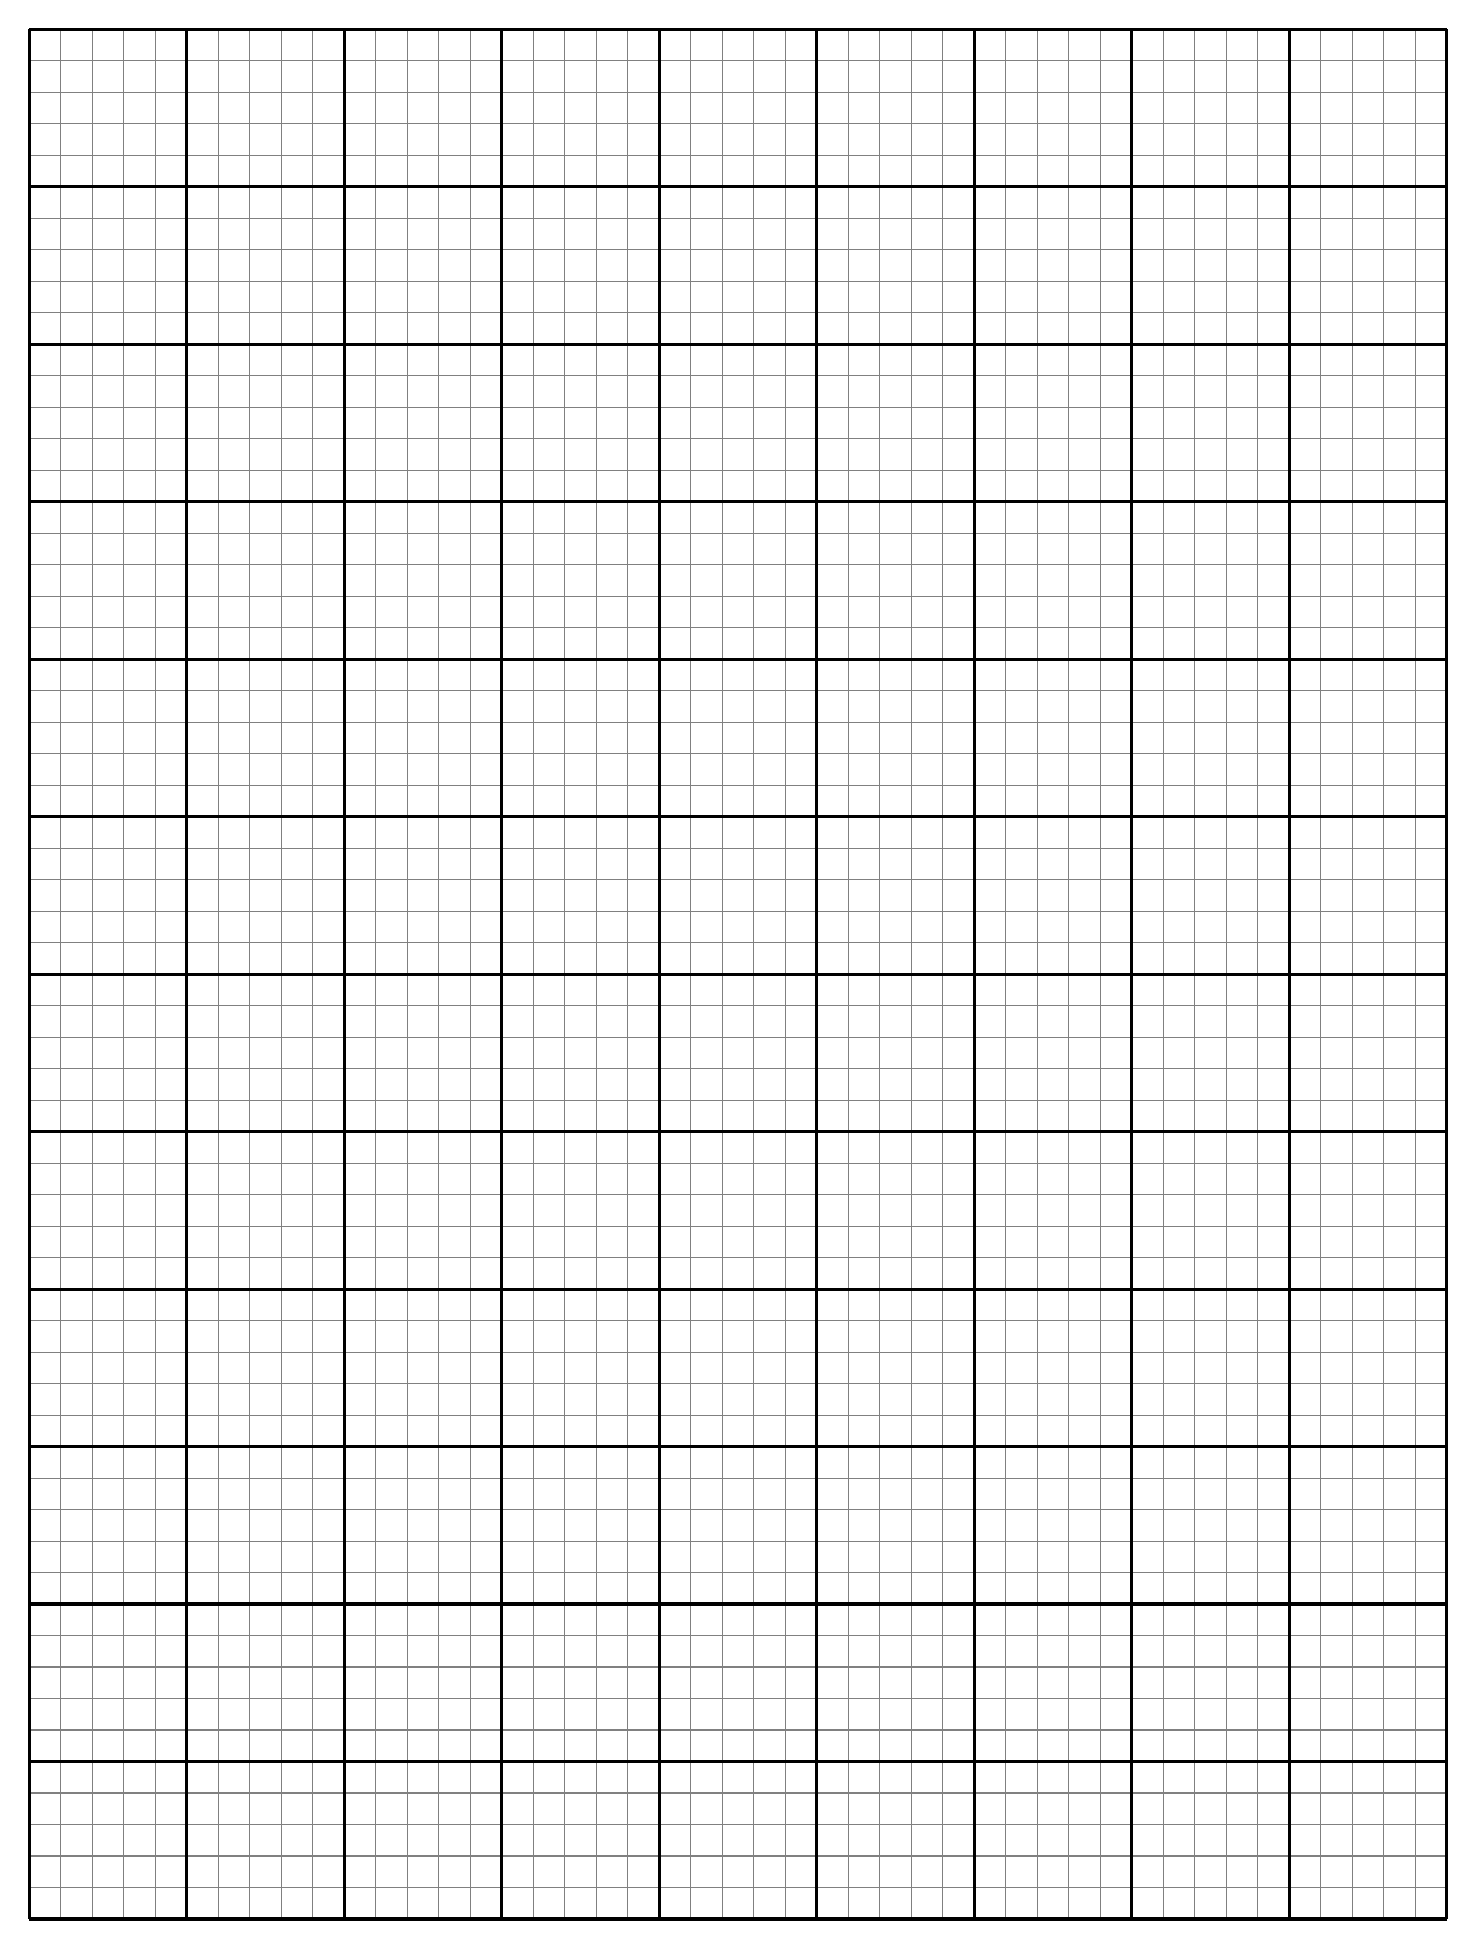
\begin{tikzpicture}[every node/.style={minimum size=1cm-\pgflinewidth, outer sep=10pt}, scale=2]
    \draw[step=0.2cm,color=gray] (0,0) grid (9,12);
    \draw[step=1cm,color=black,line width=0.4mm] (0,0) grid (9,12);
\end{tikzpicture}
